
\documentclass{sigplanconf}
\usepackage{pdf14}
\usepackage{graphicx}
\usepackage{alltt}
\usepackage{flushend}
\usepackage{style/code}
\usepackage{style/utils}

% packages for plots / tree diagrams
\usepackage{adjustbox}
\usepackage{pgfplots}
\usepackage{tikz}
\usetikzlibrary{arrows}

\colorlet{plot-orange}{red!50!orange}
\colorlet{plot-blue}{black!30!blue}
\colorlet{plot-green}{black!60!green}

% -----------------------------------------------------------------------------
\begin{document}
\toappear{}
\title
{       Gens N' Roses: Appetite for Reduction}
 
\authorinfo
{       Jacob Stanley$^\alpha$ \and 
        Charles O'Farrell$^\alpha$ \and
        Ben Lippmeier$^{\beta,\gamma}$

}
{ 
  \vspace{5pt}
  \shortstack{
    $^\alpha$Ambiata (Australia) \\
    \\[2pt]
    ~~~~~ \textsf{\{jacob.stanley, charles.ofarrell\}@ambiata.com}~~~~~~
  }
  \shortstack{
    $^{\beta}$Digital Asset (Australia) \\
    \\[2pt]
    ~~~~~~ \textsf{ben.lippmeier@digitalasset.com}~~~~~~
  }
  \shortstack{
    ~~~$^{\gamma}$UNSW (Australia) \\
    \\[2pt]
    ~~~~~~ \textsf{ben.lippmeier@unsw.edu.au}
  }
}


\maketitle
\makeatactive

% -----------------------------------------------------------------------------
\begin{abstract}
The abstract.
\end{abstract}

\category
        {D.3.4}
        {Programming Languages}
        {Processors---Compilers; Optimization}

\keywords
        Haskell; Testing


% -----------------------------------------------------------------------------
%!TEX root = ../Main.tex
\section{Introduction}

QuickCheck\cite{claessen:quickcheck} is a shockingly effective tool for validating the initial and ongoing correctness of production software. One of QuickCheck's most compelling features is that when a test failure is found, the failing test case is simplified to a minimal counterexample, through a process called shrinking. This makes it significantly easier to understand why a test has failed.

The Haskell version of QuickCheck, and its derivatives, tackle test input generation and shrinking in a type-directed fashion. This means that the programmer is required to implement an instance of the @Arbitrary@ type class for their data type in order to generate test data for it.

The @Arbitrary@ type class defines two separate methods, one for generating test inputs, and one for shrinking them. However, in practice, programmers rarely provide shrink functions for their @Arbitrary@ instances, thus losing one of QuickCheck's key benefits. Less than 20 percent of @Arbitrary@ instances on Hackage implement shrinking.

\begin{code}
  newtype Gen a =
    Gen (StdGen -> a)

  class Arbitrary a where
    arbitrary :: Gen a
    shrink    :: a -> [a]
\end{code}

Quiviq's QuickCheck for Erlang, Hypothesis for Python, and test.check for Clojure on the other hand, integrate their shrinking capability directly with test data generation. This is likely because it is the only option for dynamically typed languages, but we believe this approach is highly beneficial, even in the context of a strong statically typed language like Haskell.

\emph{Semantic Shrinking}. Shrinks should be based on the original generator, not just on the structural type. We often want to shrink to a "nice" value rather than the structurally smallest one. For example, dates can be shrunk to a value like 2000-01-01 rather than 0001-01-01. In practice we can handle this using newtype wrappers, but writing code to wrap and unwrap values is tedious. For example, consider a map from @Foo@ to @Bar@ \TODO{better example}. Some shrink don't preserve the semantic meaning of the values they are shrinking.

\emph{Splitting} of the random number generator. Shrinking the number of elements in collection structure should effect now new sub-terms are generated. \TODO{need an example}.

We make the following contributions:
\begin{itemize}
\item Our system automatically provides shrinks when constructing test data generators.

\item Our system makes it easy to provide shrink functions that take into account the semantic meaning of the data, rather than just its structural type.

\item The shrunk counterexamples produced by our system are guaranteed to be coherent(?). Relate this back to example.
\end{itemize}

%!TEX root = ../Main.tex
\section{Everything is Roses}

\TODO{Give some examples of trees}

\tikzset{
    treenode/.style = {
        circle
      , font = \sffamily
      , align = center
      , text centered
      , text width = 1.5em
      , inner sep = 0pt
      , very thick
      }
  , outcome/.style = {
        treenode
      , font = \sffamily\bfseries
      , white
      , draw = black
      , fill = black
      }
  , shrink/.style = {
        treenode
      , black
      , draw = black
      }
}

%
% I have no idea what I'm doing with this marginbox thing, it just looked weird
% without it - feel free to fix when the time comes.
%
% The nodes which have 'at (x,y)' below have slightly tweaked relative
% positions, as the default layout assumes a balanced tree, which shrink trees
% are not.
%
\marginbox{-0.5em 1em 0em 1em}{\begin{tikzpicture}[
    ->
  , > = stealth'
  , level/.style = {
        sibling distance = 3.9cm/#1
      , level distance = 1cm
      }
  ]
\node [outcome] {5}
  child {
    node [shrink] at (2,0) {0}
  }
  child {
    node [shrink] {3}
    child {
      node [shrink] {0}
    }
    child {
      node [shrink] at (-1,0) {2}
      child {
        node [shrink] {0}
      }
      child {
        node [shrink] {1}
        child {
          node [shrink] {0}
        }
      }
    }
  }
  child {
    node [shrink] at (-1.65,0) {4}
    child {
      node [shrink] at (1,0) {0}
    }
    child {
      node [shrink] {2}
      child {
        node [shrink] {0}
      }
      child {
        node [shrink] {1}
        child {
          node [shrink] {0}
        }
      }
    }
    child {
      node [shrink] at (0.3,0) {3}
      child {
        node [shrink] {0}
      }
      child {
        node [shrink] {2}
        child {
          node [shrink] {0}
        }
        child {
          node [shrink] {1}
          child {
            node [shrink] {0}
          }
        }
      }
    }
  }
;
\end{tikzpicture}}

\TODO{Not sure what text would be good here? I've knocked up the shrink tree for the integer 5.}

\begin{code}
  data Tree a =
    Node a [Tree a]
\end{code}

QuickCheck implements shrinking for properties using a rose tree. A property is just a generator which produces a tree of results. The root of the tree is the result of the randomly generated test case, while the shrinks are the sub-trees.

\begin{code}
  data Result =
    Result {
        success         :: Bool
      , counterexamples :: [String]
      }

  newtype Property =
    Property (Gen (Tree Result))
\end{code}

Lazy trees offer a very clean way to search the space of simplified test cases, but only exposing its construction to the programmer via a type class bound @shrink@ function has a number of problems.

While generators can be combined using the familiar @Functor@ / @Applicative@ / @Monad@ interface, @Arbitrary@ instances cannot. One might think that changing @Arbitrary@ to a data type might solve this problem, but unfortunately the @shrink@ function is invariant, and thus @Arbitrary@ can never be a covariant @Functor@.

\begin{code}
  data Arbitrary a =
    Arbitrary {
        arbitrary :: Gen a
      , shrink    :: a -> [a] -- invariant
      }
\end{code}

We propose that generators themselves should produce a tree. Not only does this allow generators to implement more involved shrinking strategies, the covariant nature of rose trees allows us to keep the convenient @Functor@ / @Applicative@ / @Monad@ interface which we know and love.

\TODO{Flesh this out a bit more?}

\begin{code}
  newtype Gen a =
    Gen (StdGen -> Tree a)
\end{code}

Imagine a general system for storing well-typed data, with built-in aggregation capabilities. Such a system might be used in the context of feature engineering, for a machine learning platform, such as the one we have developed at Ambiata.

In order to test the functions involved in implementing this system, one would need to generate sets of values which have compatible schemas. This is incredibly difficult using a type directed approach to generation and shrinking.

\TODO{Not sure if the aggregation part is more than necessary at this point. The fact that the values are aggregates means they are semigroups, so we can talk about merging/appending them together. It also gives us something which is in the schema, but not available in the value, so we can't derive the schema from the value.}

\begin{code}
  data Aggregate =
      Minimum
    | Maximum
    | Sum

  data Schema =
      SInt Int Int Aggregate
    | SPair Schema Schema

  data Value =
      VInt Int
    | VPair Value Value
\end{code}

If we wanted to test a function which requires two sets of values with matching schemas, the obvious thing to do is to generate a schema, then use that to generate values which comply with the schema. To do this, we will use a number of QuickCheck's @Gen@ combinators. @elements@ selects a random value from a list of options, @oneof@ executes a random generator from the input list and @choose@ generates a value in the specified range.

\begin{code}
  elements :: [a] -> Gen a

  oneof :: [Gen a] -> Gen a

  choose :: Random a => (a, a) -> Gen a
\end{code}

Implementing an @Arbitrary@ instance for this scenario requires the creation of a new data type, and the implementation of the @shrink@ function for this data type is anything but obvious.

\begin{code}
  data TwoValue =
    TwoValue Schema [Value] [Value]

  genSInt :: Gen Schema
  genSInt = do
    x <- arbitrary
    y <- arbitrary
    SInt (min x y) (max x y)
      <$> elements [Minimum, Maximum, Sum]

  genSchema :: Gen Schema
  genSchema =
    oneof [
        genSInt
      , SPair <$> genSchema <*> genSchema
      ]

  genValue :: Schema -> Gen Value
  genValue = \case
    SInt vmin vmax _ ->
      VInt <$> choose (vmin, vmax)
    SPair sx sy ->
      VPair <$> genValue sx <*> genValue sy

  instance Arbitrary TwoValue where
    arbitrary = do
      schema <- genSchema
      TwoValue schema
        <$> listOf (genValue schema)
        <*> listOf (genValue schema)
    shrink =
      -- ??? TODO should I actually write this out?

  prop_test :: TwoValue -> Property
  prop_test (TwoValue schema vs0 vs1) =
    -- some test
\end{code}

Because writing shrinkers is difficult, programmers often forgo this step entirely when writing @Arbitrary@ instances. Opting instead to use the default implementation which just returns the empty list. In some cases they may be able to use @genericShrink@, which uses @GHC.Generics@ to automatically derive a shrink function for their data type. This will not, however, take in to account invariants which a data type may have. \TODO{hackage / github results here?}

In our example, the schema @SInt@ specifies the range of values a @VInt@ can take. If we tried to use @genericShrink@ here it would happily shrink to a value which broke the invariants imposed by the schema.

Another problem with the QuickCheck version of our example is that it uses @arbitrary@ to generate @Int@ values for the @SInt@ constructor. This seems like the obvious thing to do, but the @Arbitrary@ instance for @Int@ will only generate values from @0@ to @100@. This may be fine for many situations, but in our case we'd like to test the full range of @Int@. This can easily be done in QuickCheck, but the type-directed approach to generating values entices programmers towards the wrong solution here. \TODO{this implicit decision has actually caused me a lot of pain, with generators not doing what I thought they were doing, not sure how to say this though. I've also found coworkers doing this and not realising that they weren't testing what they thought they were.}

With rose tree generators we can solve these problems. Because we need to provide shrinking as well as input generation, some of our combinators are slightly different to QuickCheck. While QuickCheck has a single @choose@ combinator for generating values in a range, we have a number of different ones. This is because we need to know more about a type in order to provide a shrinker for it.

\begin{code}
  integral :: Integral a => a -> a -> Gen a

  realFloat :: RealFloat a => a -> a -> Gen a

  enum :: Enum a => a -> a -> Gen a
\end{code}

Here are the same set of generators constructed using our approach.

\begin{code}
  genSInt :: Gen Schema
  genSInt = do
    x <- integral minBound maxBound
    y <- integral minBound maxBound
    SInt (min x y) (max x y)
      <$> elements [Minimum, Maximum, Sum]

  genSchema :: Gen Schema
  genSchema =
    oneof [
        genSInt
      , SPair <$> genSchema <*> genSchema
      ]

  genValue :: Schema -> Gen Value
  genValue = \case
    SInt vmin vmax _ ->
      VInt <$> integral vmin vmax
    SPair sx sy ->
      VPair <$> genValue sx <*> genValue sy

  prop_test :: Property ()
  prop_test = do
    schema <- forAll genSchema
    vs0 <- forAll $ listOf (genValue schema)
    vs1 <- forAll $ listOf (genValue schema)
    -- some test
\end{code}

When it comes to building up generators, the essence isn't a lot of different. However, we haven't needed to construct a data type solely for the purpose of making an @Arbitrary@ instance. In addition, because we've escewed our overloaded @arbitrary@ function for explicit combinators, it's obvious that we're testing the whole range of @Int@ when we construct an @SInt@. The key difference though, is that we haven't had to think about writing a shrink function, it comes for free, simply by combining generators. Not only that, the shrinks for our values are always guaranteed to obey our schema, by construction.

%!TEX root = ../Main.tex
\section{Ranged Generators}

QuickCheck has the notion of a \emph{size} parameter, which is varied between test case executions. Smaller sizes are tried first, before gradually increasing the size as further test cases are executed. This helps to produce smaller counterexamples as trivial inputs are tested before more complex ones. It also provides a way for the programmer to avoid diverging when generating recursive data structures. As such, our generators also accept a size parameter when generating values. \TODO{Discussed in original QuickCheck paper: 3.2 Generators for User-Defined Types}

\begin{code}
  newtype Size =
    Size Int

  newtype Gen a =
    Gen (Size -> StdGen -> Tree a)
\end{code}

Concretely, it may help to think of the size parameter as a percentage which never gets to @100@. When the test runner executes the first test case for a property, the size is @0@. The size then increases by one for each test until it gets to @99@ on the 100th test, before reseting to @0@ on the 101st test.

%
% Size vs Number of Tests
%

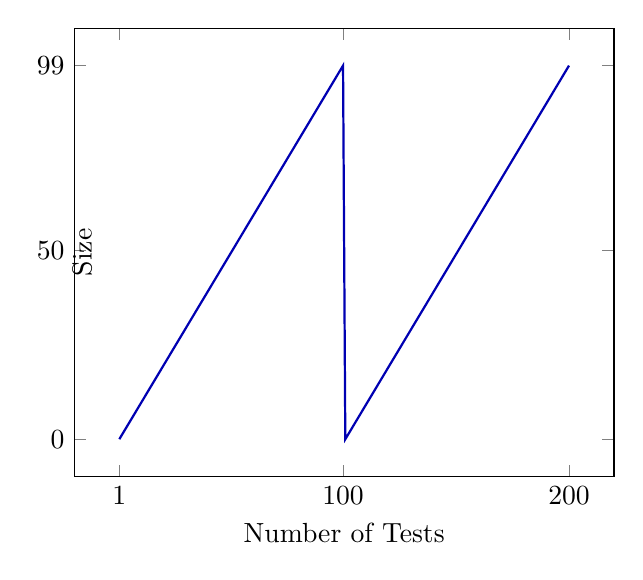
\begin{tikzpicture}
\begin{axis}[
    xlabel = Number of Tests
  , xtick = {1, 100, 200}
  , ylabel = Size
  , ytick = {0, 50, 99}
  , ylabel style = {
        at = { (0.05, 0.5) }
      }
  ]
\addplot[plot-blue, thick] plot coordinates {
  (1,0)
  (100,99)
  (101,0)
  (200,99)
};
\end{axis}
\end{tikzpicture}

Some of QuickCheck's combinators, such as @listOf@, make use of the size parameter to limit the values they generate. While others, such as @choose@ are unaffected. Unsurprisingly, none of QuickCheck's combinators offer control over how a value shrinks, because shrinking in QuickCheck is handled with the @Arbitrary@ type class.

We provide a range of combinators for controlling both how a value shrinks, and how it is affected by the size parameter. The workhorse for these combinators is the @Range@ data type.

\begin{code}
  data Range a =
    Range a (Size -> (a, a))
\end{code}

A @Range@ consists of an \emph{origin}, which is the value we would like to shrink towards, and a \emph{bounds function}, which calculates the upper and lower bound for a generator, given the current size. On top of this range abstraction, we can build a number of combinators which allow us finer control over the scope of generated values.

\begin{code}
  singleton :: a -> Range a
  singleton x =
    Range x (const (x, x))
\end{code}

@singleton@ constructs a range which always generates the same value.

\begin{code}
  constant :: a -> a -> Range a
  constant x y =
    constantFrom x x y

  constantFrom :: a -> a -> a -> Range a
  constantFrom z x y =
    Range z (const (x, y))

  constantBounded :: (Bounded a, Num a) => Range a
  constantBounded =
    constantFrom 0 minBound maxBound
\end{code}

The constant range combinators are unaffected by the size parameter. @constant@ constructs a range which shrinks to the first bound specified. Note that the bounds do not need to be specified as low then high, @constant 10 0@ is a perfectly legal application which means "generate a value between 0 and 10, shrinking towards 10". @constantFrom@ gives slightly more control, it takes an extra argument which specifies the origin to shrink towards. @constantBounded@ uses the @Bounded@ instance for a type to determine the range.

%-------------------------------------------------------------------------------
% Plots for constant/constantFrom

%
% Range.constant 0 10
%
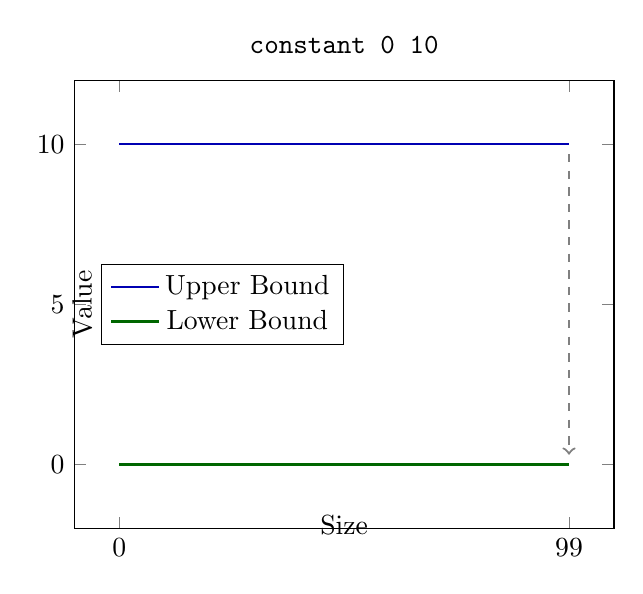
\begin{tikzpicture}
\begin{axis}[
    title = constant 0 10
  , title style = {
        font=\ttfamily
      }
  , xtick = {0, 99}
  , xlabel = Size
  , xlabel style = {
        at = { (0.5, 0.05) }
      }
  , ytick = {0, 5, 10}
  , ylabel = Value
  , ylabel style = {
        at = { (0.05, 0.5) }
      }
  , ymin = -2
  , ymax = 12
  , legend style= {
        at = { (0.05, 0.5) }
      , anchor = west
      }
  ]

\addplot[plot-blue, thick] plot coordinates {
  (0,10)
  (99,10)
};
\addlegendentry{Upper Bound}

\addplot[plot-green, thick] plot coordinates {
  (0,0)
  (99,0)
};
\addlegendentry{Lower Bound}

\node (upper)  at (axis cs:99,10) {};
\node (origin) at (axis cs:99,0) {};
\draw[->, gray, thick, dashed] (upper) -- (origin);

\end{axis}
\end{tikzpicture}

%
% Range.constantFrom 0 (-100) 100
%
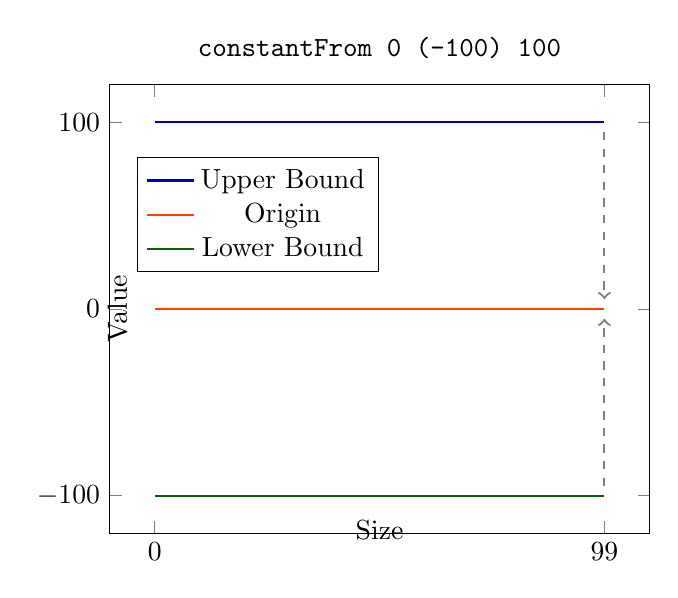
\begin{tikzpicture}
\begin{axis}[
    title = constantFrom 0 (-100) 100
  , title style = {
        font=\ttfamily
      }
  , xtick = {0, 99}
  , xlabel = Size
  , xlabel style = {
        at = { (0.5, 0.05) }
      }
  , ytick = {-100, 0, 100}
  , ylabel = Value
  , ylabel style = {
        at = { (0.05, 0.5) }
      }
  , legend style= {
        at = { (0.05, 0.71) }
      , anchor = west
      }
  ]

\addplot[plot-blue, thick] plot coordinates {
  (0,100)
  (99,100)
};
\addlegendentry{Upper Bound}

\addplot[plot-orange, thick] plot coordinates {
  (0,0)
  (99,0)
};
\addlegendentry{Origin}

\addplot[plot-green, thick] plot coordinates {
  (0,-100)
  (99,-100)
};
\addlegendentry{Lower Bound}

\node (upper)  at (axis cs:99,100) {};
\node (origin) at (axis cs:99,0) {};
\node (lower)  at (axis cs:99,-100) {};
\draw[->, gray, thick, dashed] (upper) -- (origin);
\draw[->, gray, thick, dashed] (lower) -- (origin);

\end{axis}
\end{tikzpicture}

% End plots for constant/constantFrom
%-------------------------------------------------------------------------------

\begin{code}
  linear :: Integral a => a -> a -> Range a
  linear x y =
    linearFrom x x y

  linearFrom :: Integral a => a -> a -> a -> Range a
  linearFrom z x y =
    Range z $ \size ->
      ( clamp x y (scaleLinear size z x)
      , clamp x y (scaleLinear size z y) )

  linearBounded :: (Bounded a, Integral a) => Range a
  linearBounded =
    constantFrom 0 minBound maxBound

  -- Not sure if we should include the definition
  -- of clamp and scaleLinear here?
\end{code}

The linear range combinators are similar to the constant range combinators except that their bounds scale, away from the origin, linearly with the size.

Now we have introduced range combinators, we can see how they can be used to provide better control over generated values. QuickCheck has a number of combinators for generating lists, @listOf@, @listOf1@, and @vectorOf@. These can be replaced with a single @list@ combinator, using ranges.

\begin{code}
  list :: Range Int -> Gen a -> Gen [a]

  listOf =
    list (linear 0 99)

  listOf1 =
    list (linear 1 99)

  vectorOf n =
    list (singleton n)
\end{code}

We can also go back to our @SInt@ generator, and improve the shrinking, changing @integral@ to take a @Range@ instead of two values. Now @x@ and @y@ will shrink to @0@ instead of @minBound@.

\begin{code}
  genSInt :: Gen Schema
  genSInt = do
    x <- integral linearBounded
    y <- integral linearBounded
    SInt (min x y) (max x y)
      <$> elements [Minimum, Maximum, Sum]
\end{code}

An interesting use case of range combinators is when generating gregorian calendar years. We can check a progressively larger range of years while always shrinking to a nice year, like @2000@.

\begin{code}
  genYear :: Gen Int
  genYear =
    integral (linearFrom 2000 1600 3000)
\end{code}

We could achieve this using a @newtype@ in QuickCheck, but it is far more cumbersome.

\begin{code}
  newtype Year =
    Year {
        unYear :: Int
      }

  instance Arbitrary Year where
    arbitrary =
      sized $ \n ->
        let
          lo = n * ((1600 - 2000) `quot` 99)
          hi = n * ((3000 - 2000) `quot` 99)
        in
          choose (lo, hi)

    shrink x =
      map (+ 2000) $ shrinkIntegral (x - 2000)
\end{code}

Worse still, if we wanted to use this to generate and shrink a data type from a third-party library, which doesn't happen to use our @newtype@, we'd have to wrap it then unwrap it to access the shrinking functionality.

\begin{code}
  data SomeRecord =
    SomeRecord Int

  instance Arbitrary SomeRecord where
    arbitrary =
      SomeRecord . unYear <$> arbitrary

    shrink (SomeRecord x) =
      map (SomeRecord . unYear) $ shrink (Year x)
\end{code}

With our system, this is easy.

\begin{code}
  genSomeRecord :: Gen SomeRecord
  genSomeRecord =
    SomeRecord <$> genYear
\end{code}

%-------------------------------------------------------------------------------
% Plots for linear/linearFrom

%
% Range.linear 32 1024
%
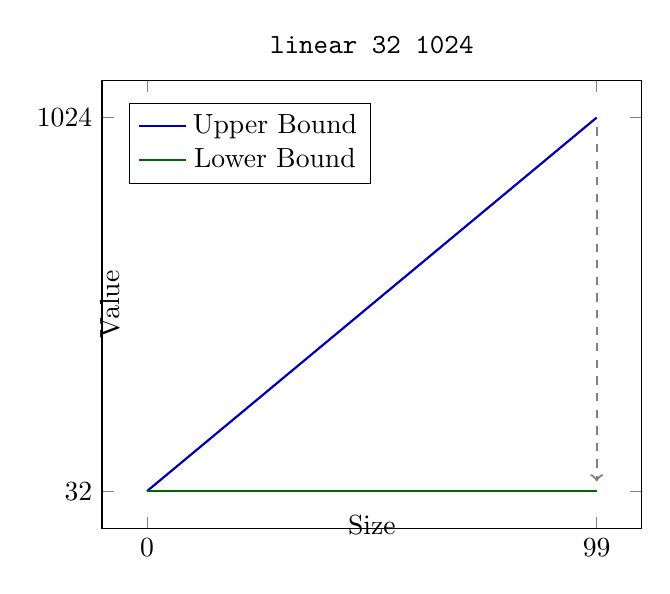
\begin{tikzpicture}
\begin{axis}[
    /pgf/number format/.cd
  , use comma
  , 1000 sep = {}
  , title = linear 32 1024
  , title style = {
        font=\ttfamily
      }
  , xlabel = Size
  , xtick = {0, 99}
  , xlabel style = {
        at = { (0.5, 0.05) }
      }
  , ylabel = Value
  , ytick = {32, 1024}
  , ylabel style = {
        at = { (0.05, 0.5) }
      }
  , legend style= {
        at = { (0.05, 0.95) }
      , anchor = north west
      }
  ]

\addplot[plot-blue, thick] plot coordinates {
  (0,32)
  (99,1024)
};
\addlegendentry{Upper Bound}

\addplot[plot-green, thick] plot coordinates {
  (0,32)
  (99,32)
};
\addlegendentry{Lower Bound}

\node (upper)  at (axis cs:99,1024) {};
\node (origin) at (axis cs:99,32) {};
\draw[->, gray, thick, dashed] (upper) -- (origin);

\end{axis}
\end{tikzpicture}

%
% Range.linearFrom 2000 1970 2100
%
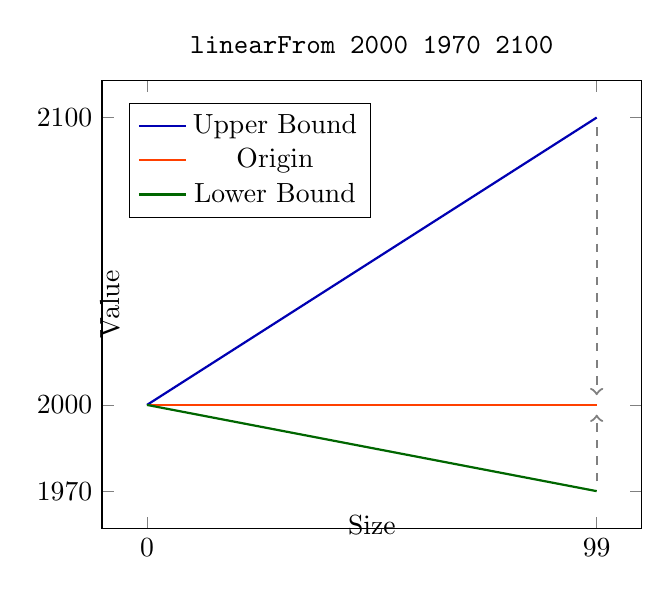
\begin{tikzpicture}
\begin{axis}[
    /pgf/number format/.cd
  , use comma
  , 1000 sep = {}
  , title = linearFrom 2000 1970 2100
  , title style = {
        font=\ttfamily
      }
  , xtick = {0, 99}
  , xlabel = Size
  , xlabel style = {
        at = { (0.5, 0.05) }
      }
  , ytick = {1970, 2000, 2100}
  , ylabel = Value
  , ylabel style = {
        at = { (0.05, 0.5) }
      }
  , legend style= {
        at = { (0.05, 0.95) }
      , anchor = north west
      }
  ]

\addplot[plot-blue, thick] plot coordinates {
  (0,2000)
  (99,2100)
};
\addlegendentry{Upper Bound}

\addplot[plot-orange, thick] plot coordinates {
  (0,2000)
  (99,2000)
};
\addlegendentry{Origin}

\addplot[plot-green, thick] plot coordinates {
  (0,2000)
  (99,1970)
};
\addlegendentry{Lower Bound}

\node (upper)  at (axis cs:99,2100) {};
\node (origin) at (axis cs:99,2000) {};
\node (lower)  at (axis cs:99,1970) {};
\draw[->, gray, thick, dashed] (upper) -- (origin);
\draw[->, gray, thick, dashed] (lower) -- (origin);

\end{axis}
\end{tikzpicture}

% End plots for linear/linearFrom
%-------------------------------------------------------------------------------

%!TEX root = ../Main.tex
\section{Effectful Generators}

One the limitations of generators in QuickCheck is that they cannot have effects. We lift this restriction by making our rose tree a monad transformer.

\begin{code}
  newtype Tree m a =
    Tree (m (Node m a))

  data Node m a =
    Node a [Tree m a]
\end{code}

This has an immediate payoff. While discards are implementing in QuickCheck using exceptions, we can simply combine our @Tree@ with a @MaybeT@. This provides discards and filtering of generators via the @Alternative@ / @MonadPlus@ class. \TODO{discuss what discards are?}

\begin{code}
  newtype Gen m a =
    Gen (Size -> StdGen -> Tree (MaybeT m) a)

  discard :: Monad m => Gen m a
  discard =
    empty -- or mzero

  filter :: Monad m => (a -> Bool) -> Gen m a -> Gen m a
  filter p gen =
    mfilter p gen <|> filter p gen
    -- actual implementation more complex
    -- to avoid looping forever

  suchThat :: Monad m => Gen m a -> (a -> Bool) -> Gen m a
  suchThat =
    flip filter
\end{code}

\TODO{Discuss generators which use @ReaderT@}

\TODO{Example of a @Gen IO@ which picks a random customer-id from a file.}

\TODO{Show that properties are @Gen m Result@, and so we get monadic testing this way.}

PureScript is a strict dialect of Haskell which compiles to JavaScript. Because it tries to keep as closely as possible to JavaScript's execution model, its runtime lacks threads of any kind. Instead it opts to provide concurrency by abstracting over continuations using the @Aff@ monad.

\begin{code}
  data Error -- JavaScript Error

  newtype Aff a =
    Aff (ExceptT Error (ContT () IO a))
\end{code}

Say we wanted to test a function which fetches a response from a url.

\begin{code}
  newtype Url =
    Url String

  newtype Response =
    Response String

  ajaxGet :: Url -> Aff Response
\end{code}

\TODO{Make sure this is a use case which QuickCheck's monadic testing won't handle elegantly.}

%!TEX root = ../Main.tex
\section{Shrinking Subterms}

One of the challenges with the rose tree approach is how to shrink a term to one of its subterms.

\TODO{describe @freeze@, @shrink@, and the @withSubterms@ combinator}

\TODO{this section probably needs to be after the transformers one as we'd like to use the @MonadPlus@ gained with @MaybeT@ to help with @list@ shrinking}

%!TEX root = ../Main.tex
\section{Upgrade}

Maybe refactor some existing libraries on hackage to use our new library. Demonstrate that we can slot in our new thing with minimal effort and make existing libraries better.


%!TEX root = ../Main.tex
\clearpage
\section{Related Work}

Sentence about QuickCheck\cite{claessen:quickcheck}. 

Cite all the related work that we have found and \emph{give a comparison} as to how that work is different to our own. If ours is better then say how.

We suspect that some other systems are implemented in this way, but it's not written up properly. Suspect that the commercial Erlang version of QuickCheck works in this way. 

There is also a Closure library that uses a rose tree, but it's not written up. Suspect that the bind implementation is wrong. Bind re-splits the tree for every shrink. Don't want to re-generate new random values when we shrink, just less of the old values. Example, when shrinking a 10 elem list the result might have 5 elems of the prev list, but not 5 entirely new elements. 

Python library has integrated shrinking but is not implemented with a rose tree.


%!TEX root = ../Main.tex
\section{Conclusion}

Give the deeper insight that we have gained when working on this project. Eg, why existing libraries are not really monadic and why ours is, and why that is better.




% -----------------------------------------------------------------------------
\bibliographystyle{plain}
\bibliography{Main}


\end{document}
